% concatenated from euler-metals.tex
\documentclass[a4paper,10pt]{article}
\usepackage[bbgreekl]{mathbbol}
\usepackage[small]{titlesec}
%\UseRawInputEncoding
\usepackage[utf8]{inputenc}
\usepackage[T1]{fontenc}  
\usepackage[]{mdframed}
\usepackage{mathrsfs}
% -----------------------------------------
% For biblatex:
%\usepackage[backend=biber,style=numeric-comp,natbib=false,giveninits=false,doi=true,isbn=false,url=false,date=year,sorting=nyvt,maxcitenames=50]{biblatex}
%\usepackage[backend=biber,style=alphabetic,natbib=false,giveninits=true,doi=true,isbn=false,url=false,date=year,maxbibnames=99,sorting=ynt,defernumbers=true]{biblatex}
\usepackage[backend=biber,style=alphabetic,natbib=false,giveninits=true,doi=true,isbn=false,url=false,date=year,maxbibnames=99,sorting=nty,defernumbers=true]{biblatex}
\DeclareNameAlias{default}{family-given}
\renewcommand{\labelnamepunct}{\addcolon\space}
\DeclareFieldFormat[article]{title}{#1}
\renewbibmacro{in:}{}
\DeclareFieldFormat[article]{pages}{#1}
\DeclareFieldFormat{journal}{#1}
\renewcommand\bf\bfseries

\renewbibmacro*{volume+number+eid}{%
	\printfield{volume}%
	%	  \setunit*{\adddot}% DELETED
	\setunit*{\addnbspace}% NEW (optional); there's also \addnbthinspace
	\printfield{number}%
	\setunit{\addcomma\space}%
	\printfield{eid}}
\DeclareFieldFormat[article]{number}{\mkbibparens{#1}}
\DeclareFieldFormat[article]{volume}{\textbf{#1}}
\DeclareFieldFormat{year}{\mkbibparens{#1}}
\DeclareBibliographyDriver{article}{%
	\printnames{author}:%
	\newunit\newblock
	\printfield{title}%
	\newunit\newblock
	\printfield{journaltitle}
	\newunit
	\iffieldundef{number}{\printfield{volume}}{\printfield{volume}\addspace\printfield{number}}
	\addcomma\addspace\printfield{pages}\addspace
	%\newunit
	\printfield{year}
	%\finentry
}
\addbibresource{euler-metals.bib}
%\usepackage{biblatex-files}
\AtEveryBibitem{\clearfield{month}}
\AtEveryBibitem{\clearfield{day}}
% -----------------------------------------
\usepackage[english]{babel}
%\usepackage[latin1]{inputenc}
\usepackage[T1]{fontenc}
\usepackage{csquotes}
\usepackage{bbm}
\usepackage[leqno]{amsmath}
\usepackage{amsfonts,amsthm,amsbsy,amssymb,dsfont,stmaryrd}
\usepackage[dvipsnames]{xcolor}
\usepackage{braket}
%\usepackage{showkeys}


\makeatletter
\newcommand{\leqnomode}{\tagsleft@true\let\veqno\@@leqno}
\newcommand{\reqnomode}{\tagsleft@false\let\veqno\@@eqno}
\makeatother


\usepackage{mathtools}
\usepackage[makeroom]{cancel}
%\mathtoolsset{showonlyrefs}

\numberwithin{equation}{section}

\newcommand\myshade{85}
\colorlet{mylinkcolor}{violet}
\colorlet{mycitecolor}{YellowOrange}
\colorlet{myurlcolor}{Aquamarine}

\usepackage[left=2.5cm,right=2.5cm,top=2.5cm,bottom=2.5cm]{geometry}
\usepackage[unicode=true,pdfusetitle,
bookmarks=true,bookmarksnumbered=false,bookmarksopen=false,
breaklinks=false,pdfborder={0 0 1},backref=false,
linkcolor  = mylinkcolor!\myshade!black,
citecolor  = mycitecolor!\myshade!black,
urlcolor   = myurlcolor!\myshade!black,
colorlinks = true,
]
{hyperref}
\usepackage[nameinlink]{cleveref}


%%%%%%%%%%%%%%%%%%%%%%%%%%

%%%%% GRAPHICS %%%%%%


\usepackage{tikz}
\usetikzlibrary{arrows}
\usetikzlibrary{intersections}

\usepackage{graphicx}
\usepackage{caption}
\usepackage{slashed}
\definecolor{ct_black}{HTML}{000000}
\definecolor{ct_orange}{HTML}{ED872D}
\definecolor{ct_purple}{HTML}{7A68A6}
\definecolor{ct_blue}{HTML}{348ABD}
\definecolor{ct_turquoise}{HTML}{188487}
\definecolor{ct_red}{HTML}{E32636}
\definecolor{ct_pink}{HTML}{CF4457}
\definecolor{ct_green}{HTML}{467821}

\definecolor{ct2_green}{HTML}{9FF781}
\definecolor{ct2_green_dark}{HTML}{088A08}



\theoremstyle{plain}
\newtheorem{thm}{\protect\theoremname}[section]
\theoremstyle{plain}
\newtheorem{lem}[thm]{\protect\lemmaname}
\theoremstyle{plain}
\newtheorem{cor}[thm]{\protect\corollaryname}
\theoremstyle{plain}
\newtheorem{prop}[thm]{\protect\propositionname}
\theoremstyle{plain}
\newtheorem{claim}[thm]{\protect\claimname}



\newtheorem{assumption}[thm]{\protect\assumptionname}


\theoremstyle{remark}
\newtheorem{rem}[thm]{\protect\remarkname}


\theoremstyle{definition}
\newtheorem{defn}[thm]{\protect\definitionname}
\theoremstyle{plain}
\newtheorem{example}[thm]{\protect\examplename}
\providecommand{\assumptionname}{Assumption}
\providecommand{\claimname}{Claim}
\providecommand{\corollaryname}{Corollary}
\providecommand{\definitionname}{Definition}
\providecommand{\lemmaname}{Lemma}
\providecommand{\propositionname}{Proposition}
\providecommand{\remarkname}{Remark}
\providecommand{\theoremname}{Theorem}
\providecommand{\examplename}{Example}

\crefname{section}{Section}{Sections}
\crefname{appendix}{Appendix}{Appendices}
\crefname{figure}{Figure}{Figures}
\crefname{assumption}{Assumption}{Assumptions}
\crefname{thm}{Theorem}{Theorems}
\crefname{lem}{Lemma}{Lemmas}
\crefformat{equation}{(#2#1#3)}
\crefname{table}{Table}{Tables}

%\crefname{equation}{equation}{equations}
%\Crefname{equation}{Equation}{Equations}% For beginning \Cref
\crefrangelabelformat{equation}{(#3#1#4--#5#2#6)}

\crefmultiformat{equation}{(#2#1#3}{, #2#1#3)}{#2#1#3}{#2#1#3}
\Crefmultiformat{equation}{(#2#1#3}{, #2#1#3)}{#2#1#3}{#2#1#3}


\newtheorem*{lem*}{\protect\lemmaname}

% ############# MATH SHORTCUTS 
\newcommand{\LOC}[1]{\mathrm{LOC}_{#1}}
\newcommand{\ee}{\operatorname{e}}
\newcommand{\ii}{\operatorname{i}}
\newcommand{\Mat}{\operatorname{Mat}}
\newcommand{\Herm}{\operatorname{Herm}}
\newcommand{\ZZ}{\mathbb{Z}}
\newcommand{\TT}{\mathbb{T}}
\newcommand{\bS}{\mathbb{S}}
\newcommand{\HSSH}{H_{_{\rm SSH}}}
\newcommand{\tin}{t_{_{\rm in}}}
\newcommand{\tout}{t_{_{\rm out}}}
\newcommand{\din}{d_{_{\rm in}}}
\newcommand{\dout}{d_{_{\rm out}}}
\newcommand{\wA}{w_A}
\newcommand{\wB}{w_B}

\newcommand{\NN}{\mathbb{N}}
\newcommand{\RR}{\mathbb{R}}
\newcommand{\QQ}{\mathbb{Q}}
\newcommand{\CC}{\mathbb{C}}
\newcommand{\FF}{\mathbb{F}}
\newcommand{\PP}{\mathbb{P}}
\newcommand{\EE}{\mathbb{E}}
\newcommand{\VV}{\mathbb{Var}}
\newcommand{\calA}{\mathcal{A}}
\newcommand{\calB}{\mathcal{B}}
\newcommand{\calC}{\mathcal{C}}
\newcommand{\calF}{\mathcal{F}}
\newcommand{\calN}{\mathcal{N}}
\newcommand{\calG}{\mathcal{G}}
\newcommand{\calO}{\mathcal{O}}
\newcommand{\calR}{\mathcal{R}}
\newcommand{\calD}{\mathcal{D}}
\newcommand{\calV}{\mathcal{V}}
\newcommand{\calU}{\mathcal{U}}
\newcommand{\calSU}{\mathcal{SU}}
\newcommand{\calSG}{\mathcal{SG}}
\newcommand{\calH}{\mathcal{H}}
\newcommand{\calM}{\mathcal{M}}
\newcommand{\calK}{\mathcal{K}}
\newcommand{\calL}{\mathcal{L}}
\newcommand{\scrL}{\mathscr{L}}
\newcommand{\calI}{\mathcal{I}}
\newcommand{\calJ}{\mathcal{J}}
\newcommand{\calP}{\mathcal{P}}
\newcommand{\calS}{\mathcal{S}}
\newcommand{\Ord}[1]{\calO\left(#1\right)}
\newcommand{\Gras}[2]{\operatorname{Gr}_{#1}(#2)}
\newcommand{\Compacts}[1]{\mathcal{K}(#1)}
\newcommand{\bbLambda}{\mathbb{\Lambda}}
\newcommand{\bbDelta}{\mathbb{\Delta}}
\newcommand{\bbPsi}{\mathbb{\Psi}}
\newcommand{\bbPhi}{\mathbb{\Phi}}
\newcommand{\bbGamma}{\mathbb{\Gamma}}
\newcommand{\bbTheta}{\mathbb{\Theta}}
\newcommand{\bbSigma}{\mathbb{\Sigma}}
\newcommand{\ti}[1]{\widetilde{#1}} 
\newcommand{\LamNT}{\Lambda\mathrm{nt}}
\newcommand{\LamNTSAU}{\calSU^{\LamNT}}

\newcommand{\Fredholms}[1]{\mathcal{F}(#1)}
\newcommand{\Unitaries}[1]{\mathcal{U}(#1)}
\newcommand{\Automorphisms}[1]{\operatorname{Aut}(#1)}
\newcommand{\Endomorphisms}[1]{\operatorname{End}(#1)}
%\newcommand{\norm}[1]{\|#1\|}
\newcommand\norm[1]{\left\lVert#1\right\rVert}
%\newcommand\abs[1]{\left|#1\right|}
\newcommand{\ip}[2]{\langle #1, #2 \rangle}
\newcommand{\HSip}[2]{\langle #1, #2 \rangle_{\mathrm{HS}}}
\newcommand{\finset}[1]{\Set{1,\dots,#1}}
\DeclareMathOperator*{\slim}{s-lim}
\newcommand{\dif}{\operatorname{d}\!} % shorten the space afterwards
\newcommand{\tr}{\operatorname{tr}}


\newcommand{\szpan}{\operatorname{span}}


%\renewcommand{\Im}{\operatorname{\mathbb{I}\mathbbm{m}}}
\renewcommand{\Im}[1]{\operatorname{\mathbb{I}\mathbbm{m}}\{#1\}}
\renewcommand{\Re}[1]{\operatorname{\mathbb{R}\mathbbm{e}}\{#1\}}
\newcommand{\ve}{\varepsilon}
\newcommand{\vf}{\varphi}
\newcommand{\Id}{\mathds{1}}
% Specific shortcuts here
\newcommand{\HH}{\mathbb{H}}

\newcommand{\EH}{\HH^\sharp}
\newcommand{\BLO}[1]{\mathcal{B}(#1)}
\newcommand{\Open}[1]{\mathrm{Open}(#1)}
\newcommand{\Closed}[1]{\mathrm{Closed}(#1)}
%\newcommand{\dist}[1]{\mathrm{dist}(#1)}
\newcommand{\dist}{\mathrm{dist}}
\newcommand{\BorelSA}[1]{\mathcal{B}(#1)}
\newcommand{\quotes}[1]{``#1''}


%\newcommand{\BLO}{\mathcal{B}(\HH)}
\newcommand{\Chern}{\operatorname{Ch}}

% Macros from chiral-1d-loc paper
\newcommand{\HSG}{Sp_{2N}^\ast(\mathbb{C})}
\newcommand{\toitself}{\mathbin{\scalebox{.85}{%
			\lefteqn{\scalebox{.5}{$\blacktriangleleft$}}\raisebox{.34ex}{$\supset$}}}}

% Macros from chiral-1d-bec paper
\newcommand{\sgn}{\operatorname{sgn}}
\newcommand{\findex}{\operatorname{ind}}
\newcommand{\safindex}{\operatorname{ind}_2}
\newcommand{\rank}{\operatorname{rank}}
\newcommand{\diag}{\operatorname{diag}}
\newcommand{\coker}{\operatorname{coker}}
\newcommand{\supp}{\operatorname{supp}}
\renewcommand{\vec}[1]{\mathbf{#1}}


% Macros from Floquet paper


\DeclarePairedDelimiter\ceil{\lceil}{\rceil}
\DeclarePairedDelimiter\floor{\lfloor}{\rfloor}



\newcommand{\im}{\operatorname{im}}
\newcommand{\ad}{\operatorname{ad}}

\newcommand{\SO}{\bS^1}






\newcommand{\illim}[1]{\raisebox{0.5ex}{\scalebox{0.8}{$\displaystyle \lim_{#1}\;$}}}



\newcommand{\vm}{|v_{min}|}
\newcommand{\vmh}{\nu}

\newcommand{\corr}{\color{red}}
\newcommand{\nc}{\normalcolor}
\newcommand{\Cpt}{\Compacts{\calH}}






\usepackage{environ}

\NewEnviron{malign}{%
	\begin{align}\begin{split}
			\BODY
	\end{split}\end{align}
}






%\usepackage{refcheck}






\newcommand{\prob}[1]{\PP\left[\Set{#1}\right]}
\newcommand{\ex}[1]{\EE\left[#1\right]}
\newcommand{\HSn}[1]{\norm{#1}_{\mathrm{HS}}}



\newcommand{\eq}[1]{\begin{align*}#1\end{align*}}
\newcommand{\eql}[1]{\begin{align}#1\end{align}}
\newcommand{\mybox}[2]{\begin{mdframed}[backgroundcolor=gray!40,shadow=true,roundcorner=8pt,frametitle={#1}]#2\end{mdframed}}




\newcommand{\Projections}[1]{\mathcal{P}(#1)}
\newcommand{\Calkin}[1]{\mathcal{C}(#1)}
\newcommand{\CalkinProjections}[1]{\mathcal{Q}(#1)}

\newcommand{\polar}{\operatorname{pol}}

\newcommand{\calT}{\mathcal{T}}
\newcommand{\onehalf}{\frac{1}{2}}
\newcommand{\DD}{\mathbb{D}}
\newcommand{\Schur}{Z}







% bijection arrow 
\newcommand{\hookdoubleheadrightarrow}{%
  \hookrightarrow\mathrel{\mspace{-15mu}}\rightarrow
}





\usepackage{tikz}
\newcommand*\circled[1]{\tikz[baseline=(char.base)]{
            \node[shape=circle,draw,inner sep=2pt,color=black] (char) {#1};}}


% don't include subsections in ToC

\setcounter{tocdepth}{2} % set 2 to include subsections







%%%%%%%%%%%%%%%%%%%%

%%%%% METADATA %%%%%

\title{Euler Topological Metals in 1D}
\author{\href{mailto:jc1220@math.princeton.edu}{Yichen Hu}\\
	{\footnotesize Department of Physics, Florida Atlantic University}\\
	\href{mailto:shapiro@math.princeton.edu}{Jacob Shapiro}\\
	{\footnotesize Department of Mathematics, Princeton University}
}





%%%%%%%%%%%%%%%%%%%%


\begin{document}
	\reqnomode
	
	\maketitle
	\begin{abstract}
		We give a rigorous one-dimensional formulation of Kane's transport proposal for probing the Euler characteristic of a Fermi sea. For a clean, translation-invariant continuum Hamiltonian with real-analytic dispersion, a Fermi sea confined to a finite momentum range, and nonzero Fermi velocity at every Fermi point, we analyze a particular Abel-regularized transport response (obtained by tracing over the Fermi sea) and prove that its large-time limit equals the Euler characteristic. We derive an explicit finite-time formula, show that quantization requires the large-time limit, and obtain a convergence rate under additional nonstationarity assumptions. We also prove the lattice analog, where the sharp commutator is trace-class and a completely filled band contributes zero. Finite-volume calculations illustrate the prescribed order of the thermodynamic and large-time limits.
	\end{abstract}
	%\tableofcontents
	\section{Introduction}
    Topological phenomena in condensed matter physics are most commonly
    associated with gapped phases, where an invariant of the occupied Bloch
    bundle, such as a Chern number, is detected by a quantized transport
    coefficient \cite{Hasan_Kane_2010}. Metals have no such spectral gap, but
    they possess another natural geometric object: the occupied region in
    momentum space. Changes in the topology of this region are the classical
    Lifshitz transitions, whose thermodynamic and kinetic signatures have long
    been studied \cite{Lifshitz1960,BlanterEtAl1994}. What had been missing was
    a direct observable which returns a topological invariant of the Fermi sea
    itself.

    Kane proposed such an observable in his 2021 preprint, highlighted at the
    time by Beenakker \cite{Beenakker2021Euler}, and subsequently published in
    \cite{Kane_22_PhysRevLett.128.076801}. The proposal extends the familiar
    one-dimensional Landauer conductance \cite{Landauer1957}. In one dimension
    the number of occupied ballistic channels is the number of components of
    the Fermi sea and hence its Euler characteristic. Kane showed that in two
    dimensions the corresponding invariant is obtained instead from a
    second-order, three-terminal response: electron-like Fermi surfaces and
    hole-like Fermi surfaces enter with opposite signs. More generally, the
    proposal suggests a hierarchy in which a $d$-dimensional Fermi sea is
    probed by a $d$th-order response of $d+1$ regions meeting at a point. The
    cases $d=1,2$ were established in \cite{Kane_22_PhysRevLett.128.076801};
    the higher-dimensional transport problem was left open.

    Several subsequent works developed different aspects of this idea. Yang
    and Zhai proposed a two-dimensional ultracold-atom implementation and
    quantified the effects of finite pulses, temperature, and trap geometry
    \cite{YangZhai2022}. Zhang formulated a one-dimensional linear response in
    a trapped gas and its nonlinear higher-dimensional analogues
    \cite{Zhang2023}. Tam, Claassen, and Kane found that the same Euler
    characteristic controls a multipartite entanglement quantity associated
    with $d+1$ regions: for odd $d$ this is a multipartite mutual information,
    while for even $d$ a charge-weighted version is required
    \cite{TamClaassenKane2022}. In a different direction, Andreev bound states
    in a long Josephson junction furnish a rectified transport probe in two
    dimensions \cite{TamKane2023Andreev,TamDeBeuleKane2023}, and the Fermi-sea
    Euler characteristic can be inherited by the invariant of a weak-pairing
    topological superconductor \cite{YangLiLi2023,Jia2025}.

    Equal-time correlations provide a further formulation which is not tied
    to transport. The connected $(d+1)$-point density correlation of a free
    Fermi gas has a universal long-wavelength term proportional to the Euler
    characteristic \cite{TamKane2024}. This prediction was recently tested in
    a two-dimensional gas of ${}^{6}\mathrm{Li}$ using single-atom-resolved
    measurements of three- and four-point correlations
    \cite{DaixEtAl2025}. The limitations of the quantization are now also
    becoming visible: Berry curvature preserves the homogeneous
    two-dimensional transport formula but, together with spatial
    inhomogeneity, produces a non-quantized correction \cite{YangLi2026}; and
    in an interacting two-dimensional Fermi liquid the singular three-point
    correlation survives with a coefficient renormalized by the Landau
    parameters \cite{TamKane2026,Kane2026ThreePoint}.

    These developments show that the Euler characteristic is not exclusively
    a transport invariant. It may appear in nonlinear response, in equal-time
    density correlations and charge fluctuations \cite{TamEtAl2026ChargeFluctuations}, or in specially arranged entanglement quantities.
    The last qualification is important. The leading bipartite entanglement
    entropy of a Fermi sea is governed by a Widom-type geometric integral over
    the real-space boundary and the Fermi surface
    \cite{GioevKlich2006}; it does not by itself isolate the Euler
    characteristic. The topological term emerges only after a multipartite
    combination, and in even dimensions after charge weighting.

    The purpose of the present paper is narrower. We give a mathematical
    formulation of the one-dimensional continuum response underlying Kane's
    argument. A continuous-translation-invariant single-particle Hamiltonian
    on $L^2(\RR^d)$ is of the form
    \eq{H=f(P),\qquad P=-\ii\nabla\,,}
    and at Fermi energy $E_F$ its Fermi sea is
    \eq{\Sigma_{E_F}:=\Set{p\in\RR^d\mid f(p)\leq E_F}\,.}
    We assume below that the one-dimensional dispersion $f:\RR\to\RR$ is real analytic, that
    $E_F$ is a regular value, and that $\Sigma_{E_F}$ is compact. In one
    dimension $\chi(\Sigma_{E_F})=b_0(\Sigma_{E_F})$ is simply the number of
    its connected components. In two dimensions it is
    $b_0(\Sigma_{E_F})-b_1(\Sigma_{E_F})$, where $b_1(\Sigma_{E_F})$ is the number of holes. For general $d$ one has \eql{\chi(\Sigma_{E_F}) = \sum_{j=0}^d (-1)^{j}b_j(\Sigma_{E_F})} where $b_j(\Sigma_{E_F})$ is the $j$th Betti number of the Fermi sea.

    Even in one dimension, the formal Kubo expression contains sharp spatial
    switches and is not an ordinary trace in infinite volume. Our main result,
    \cref{thm:main theorem}, identifies an Abel-regularized and
    Fermi-compressed linear response whose large-time limit equals
    $\chi(\Sigma_{E_F})$. We also quantify why the large-time limit is
    necessary and give the analogous argument for a lattice Hamiltonian in
    \cref{sec:discrete}.

    The higher-dimensional questions remain substantial. In two dimensions
    one would like a rigorous nonlinear Kubo formula for three intersecting
    spatial switches, with a controlled infinite-volume regularization and
    order of limits. In three dimensions it is not yet clear which transport
    geometry produces the Euler characteristic, or whether a genuinely linear
    response with a more elaborate observable can replace the expected
    third-order response. More generally, it remains to determine which of the
    transport, density-correlation, and multipartite-entanglement formulations
    survive disorder and interactions, and whether their quantized terms are
    different realizations of a single index theorem.

    
    This paper is organized as follows.  In \cref{sec:continuum} we derive the formal Kubo response, identify the trace-class obstruction in the continuum, and state our regularized formulation.  After giving semiclassical and Boltzmann motivations, we prove the main theorem by direct momentum-space analysis and quantify the approach to the quantized large-time limit.  In \cref{sec:discrete} we establish the corresponding lattice result, where the sharp commutator is already trace-class and a completely filled band contributes zero.  Finally, \cref{sec:numerics} illustrates the finite-time and finite-volume effects, the role of boundary conditions, and the behavior of the response for the one-dimensional Anderson model.
\section{The one-dimensional theory}\label{sec:continuum}
    
    \subsection{The experimental setup--formal manipulations}

Consider a non-interacting electron in a continuous one-dimensional infinite
wire, with single-particle Hilbert space $L^2(\RR)$. We work in units
$\hbar=1$ and write $-e$, with $e>0$, for the electric charge of the
electron. Let
\eq{\Lambda(x):=\chi_{(0,\infty)}(x)\,.}

At time $t_0\in\RR$, we apply the scalar-potential impulse
\eq{\phi(x,t)=-\frac{E_0}{e}\Lambda(x)\delta(t-t_0),
\qquad E_0>0\,.}
The corresponding electric field and single-particle perturbation are
\eq{\mathcal{E}(x,t)
=-\partial_x\phi(x,t)
=\frac{E_0}{e}\delta(x)\delta(t-t_0)}
and
\eq{H(t)=H+E_0\Lambda(X)\delta(t-t_0)\,.}
Thus the space-time integrated electric field is $E_0/e$.

The observable
\eq{N_R:=\Lambda(X)}
measures the number of particles on the right half-line, while the
corresponding electric-charge observable is
\eq{Q_R:=-e\Lambda(X)\,.}
Indeed, the expected particle number in a region $S\subseteq\RR$ is
$\tr(\rho\chi_S(X))$. At zero temperature, the unperturbed one-particle
density matrix $\rho$ is the Fermi projection
\eq{P_F:=\chi_{(-\infty,E_F)}(H)\,.}

In finite volume, Kubo's formula
\cite{Kubo_57_I_doi:10.1143/JPSJ.12.570,
Kubo_57_II_doi:10.1143/JPSJ.12.1203,Bruus2004-lk}
gives, to first order in $E_0$,
\eql{\tr\left((\rho(t)-P_F)B\right)
&=-\ii E_0\int_{-\infty}^{t}\dif{t'}\,
\tr\left(
\ee^{-\ii(t-t')H}
\left[\Lambda(X)\delta(t'-t_0),P_F\right]
\ee^{\ii(t-t')H}B
\right)
+\calO(E_0^2)\notag\\
&=-\ii E_0\chi_{(0,\infty)}(t-t_0)
\tr\left(
\ee^{-\ii(t-t_0)H}
[\Lambda(X),P_F]
\ee^{\ii(t-t_0)H}B
\right)
+\calO(E_0^2)\,.
\label{eq:Kubo}}

Taking $B=N_R=\Lambda(X)$ and using $[H,P_F]=0$, formal cyclicity of the
trace gives
\eq{\tr\left(
\ee^{-\ii(t-t_0)H}
[\Lambda(X),P_F]
\ee^{\ii(t-t_0)H}\Lambda(X)
\right)
=
-\tr\left(
P_F\left[
\ee^{-\ii(t-t_0)H}\Lambda(X)\ee^{\ii(t-t_0)H},
\Lambda(X)
\right]
\right).}
Consequently, the formal particle-number response is
\eq{\Delta N_R(t)
:=\tr\left((\rho(t)-P_F)\Lambda(X)\right)
=
\ii E_0\chi_{(0,\infty)}(t-t_0)
\tr\left(
P_F\left[
\ee^{-\ii(t-t_0)H}\Lambda(X)\ee^{\ii(t-t_0)H},
\Lambda(X)
\right]
\right)
+\calO(E_0^2)\,.}

The electric-charge response has the opposite sign because $Q_R=-eN_R$:
\eq{\frac{2\pi}{eE_0}\Delta Q_R(t)
=
-2\pi\ii\chi_{(0,\infty)}(t-t_0)
\tr\left(
P_F\left[
\ee^{-\ii(t-t_0)H}\Lambda(X)\ee^{\ii(t-t_0)H},
\Lambda(X)
\right]
\right)
+\calO(E_0)\,.}
This is the origin of both the sign and the factor $2\pi$ in the response
considered below.

There are two obstructions to interpreting the preceding expressions as
ordinary infinite-volume traces. First, $P_F\Lambda(X)$ is not trace-class,
so the equilibrium charge on the half-line is infinite. Second, the
operators occurring in the linear term need not be trace-class, and hence
the cyclicity used above is not justified. These manipulations are therefore
only used to identify the quantity that must be regularized.

For $\ve>0$, replace the sharp switch by
\eq{\Lambda_\ve(x):=\chi_{(0,\infty)}(x)\ee^{-\ve x}}
and compress the commutator by $P_F$ on both sides. For this regularized
expression, the trace is well-defined and
\eq{&-2\pi\ii\tr\left(
P_F\left[
\ee^{-\ii(t-t_0)H}\Lambda_\ve(X)\ee^{\ii(t-t_0)H},
\Lambda_\ve(X)
\right]P_F
\right)\\
&\qquad=
2\pi\ii\tr\left(
P_F\left[
\ee^{\ii(t-t_0)H}\Lambda_\ve(X)\ee^{-\ii(t-t_0)H},
\Lambda_\ve(X)
\right]P_F
\right).}
Indeed, this follows by conjugating the first commutator by
$\ee^{\ii(t-t_0)H}$, using $[H,P_F]=0$, and applying cyclicity to the
resulting trace-class operator. Thus the backward time evolution produced
by Kubo's formula, together with the minus sign from the electron charge,
agrees exactly with the forward time evolution and positive normalization
in \cref{thm:main theorem}.

For notational convenience, from now on we take $t_0=0$ and consider the
limit $t\to\infty$.

We analyze this particular regularized response functional; we do not derive
it here as a thermodynamic limit of the finite-volume Kubo expression or
prove that it is independent of the choice of regularization.









\begin{rem}[Trace class in the continuum]
\label{rem:continuum trace class}
In the continuum, smoothness of the dispersion relation is not enough to
make the relevant commutator trace-class. What matters is also its behavior
over the entire momentum axis.

A theorem of Peller
\cite[Theorem~5.7]{Peller2024Besov}, applied after Fourier transform,
has the following simple consequence: if
\eq{
\left[\Lambda(X),\ee^{-\ii t f(P)}\right]\in\calJ_1
}
for some fixed $t\neq 0$, then the phase
$p\mapsto\ee^{-\ii t f(p)}$ must have finite total variation. For a
differentiable real-valued dispersion, this requires
\eq{
\int_{\RR}\dif{p}\,
\left|\partial_p\ee^{-\ii t f(p)}\right|
=
|t|\int_{\RR}\dif{p}\,|f'(p)|
<\infty.
}
This condition already rules out the usual proper dispersions satisfying
$f(p)\to+\infty$ as $p\to\pm\infty$: such a function necessarily has
infinite total variation. This remains true no matter how smooth or
analytic $f$ is.

For example, for the free-particle dispersion $f(p)=p^2$,
\eq{
\int_{\RR}\dif{p}\,
\left|\partial_p\ee^{-\ii t p^2}\right|
=
2|t|\int_{\RR}\dif{p}\,|p|
=
\infty.
}
Consequently, for every $t\neq 0$,
\eq{
\left[\Lambda(X),\ee^{-\ii tP^2}\right]\notin\calJ_1.
}
Thus the standard locality argument based on the trace-classness of
$\left[\Lambda(X),\ee^{-\ii tH}\right]$ is unavailable for the usual
continuum Hamiltonians. This is why \cref{thm:main theorem} instead uses
a regularized switch and compresses the commutator to the Fermi sea.

For completeness, Peller's exact criterion in the present setting is
\eql{
\left[\Lambda(X),\ee^{-\ii t f(P)}\right]\in\calJ_1
\quad\Longleftrightarrow\quad
\int_{\RR}\frac{\dif{h}}{|h|^2}
\int_{\RR}\dif{p}\,
\left|
\ee^{-\ii t f(p+2h)}
-2\ee^{-\ii t f(p+h)}
+\ee^{-\ii t f(p)}
\right|
<\infty.
\label{eq:Peller criterion}
}
The main point is that this is a global condition in momentum, rather
than a local smoothness condition.

A convenient, although stronger than necessary, sufficient assumption is
that, for some constant $c$,
\eq{
\int_{\RR}
\left(
|f(p)-c|+|f'(p)|+|f''(p)|
\right)\dif{p}
<\infty.
}
Equivalently, $f-c\in W^{2,1}(\RR)$. Under this assumption,
$\ee^{-\ii t f}-\ee^{-\ii t c}\in W^{2,1}(\RR)$, and Peller's criterion
shows that the commutator is trace-class for every fixed $t$.
\end{rem}








    
    \subsection{The main theorem}

    % For $\ve>0$ we regularize the spatial switch directly by
    % \eql{\Lambda_\ve(x):=\chi_{(0,\infty)}(x)\ee^{-\ve x}\,.}
    % Thus $\Lambda_\ve(X)\to\Lambda(X)$ strongly as $\ve\to0^+$.

    Our main theorem will be 
    \begin{thm}[The regularized response is the Euler characteristic]\label{thm:main theorem}
        Let $H=f(P)$, where $f:\RR\to\RR$ is real analytic. Assume that $E_F$ is a regular value of $f$ and that the Fermi sea
        \eql{\label{eq:Fermi sea}\Sigma_{E_F}=\Set{p\in\RR | f(p)\leq E_F}\,.}
        is compact. Then the regularized dimensionless response equals the Euler characteristic
        \eql{\lim_{t\to\infty}\lim_{\ve\to0^+}
2\pi\ii\tr\left(
P_F\left[
\ee^{\ii tH}\Lambda_\ve(X)\ee^{-\ii tH},
\Lambda_\ve(X)
\right]P_F
\right)
=\chi(\Sigma_{E_F})\,.
\label{eq:linear response}}
        
    \end{thm}
The large-time limit is essential: the finite-time response is not
topologically quantized; see \cref{prop:finite-time response} below.

\begin{proof}[Semiclassical "proof"]
We use the forward Heisenberg evolution and the prefactor $2\pi\ii$ appearing in \cref{eq:linear response}.  Suppose that
\eq{\Sigma_{E_F}=\bigsqcup_{j=1}^{N}[a_j,b_j]\,.}
The Hamiltonian flow generated by $f(p)$ is
\eq{(x,p)\longmapsto\left(x+t f'(p),p\right)\,,}
so the principal symbol of
$\ee^{\ii tH}\Lambda_\ve(X)\ee^{-\ii tH}$ is
$\Lambda_\ve(x+t f'(p))$.  Using
\eq{\{a,b\}=\partial_xa\,\partial_pb-\partial_pa\,\partial_xb}
and the semiclassical correspondence $[A,B]\sim\ii\{a,b\}$, we obtain
\eq{&
\left[\ee^{\ii tH}\Lambda_\ve(X)\ee^{-\ii tH},
\Lambda_\ve(X)\right]\\
&\qquad\sim
\ii\left\{\Lambda_\ve(x+t f'(p)),\Lambda_\ve(x)\right\}\\
&\qquad=
-\ii t f''(p)\Lambda_\ve'(x+t f'(p))\Lambda_\ve'(x)\,.}

The semiclassical trace rule, together with the symbol
$\chi_{\Sigma_{E_F}}(p)$ of $P_F$, then gives
\eq{&
2\pi\ii\tr\left(
P_F\left[
\ee^{\ii tH}\Lambda_\ve(X)\ee^{-\ii tH},
\Lambda_\ve(X)
\right]P_F
\right)\\
&\qquad\sim
\int_{\Sigma_{E_F}}\dif{p}\int_{\RR}\dif{x}\,
t f''(p)\Lambda_\ve'(x+t f'(p))\Lambda_\ve'(x)\\
&\qquad=
\int_{\Sigma_{E_F}}\dif{p}\int_{\RR}\dif{x}\,
\partial_p\Lambda_\ve(x+t f'(p))\Lambda_\ve'(x)\\
&\qquad=
\sum_{j=1}^{N}\int_{\RR}\dif{x}\,\Lambda_\ve'(x)
\left(
\Lambda_\ve(x+t f'(b_j))
-\Lambda_\ve(x+t f'(a_j))
\right)\,.}

As $\ve\to0^+$, one has
$\Lambda_\ve\to\Lambda$ and
$\Lambda_\ve'\to\delta_0$ distributionally.  Since $E_F$ is a regular value,
\eq{f'(a_j)<0,\qquad f'(b_j)>0\,,}
and hence, for every $t>0$,
\eq{&
\lim_{\ve\to0^+}
2\pi\ii\tr\left(
P_F\left[
\ee^{\ii tH}\Lambda_\ve(X)\ee^{-\ii tH},
\Lambda_\ve(X)
\right]P_F
\right)\\
&\qquad\sim
\sum_{j=1}^{N}
\left(
\Lambda(t f'(b_j))-\Lambda(t f'(a_j))
\right)
=N\,.}
The semiclassical expression is already independent of $t>0$, so its
large-time limit gives the Euler characteristic of $\Sigma_{E_F}$.
This is not a proof, since the sharp switch has a singular symbol and the
semiclassical trace rule is not controlled uniformly as $\ve\to0^+$;
justifying this singular interface contribution requires precisely the
Wiener--Hopf trace formula, or equivalently the direct momentum-space
analysis, established in the actual proof below.
\end{proof}

    
    Before we turn to the actual proof of the theorem, let us motivate it using the Boltzmann equation.

    
    \subsection{Kane's Heuristics via the Boltzmann equation}
    The collisionless Boltzmann equation gives a semiclassical explanation of the normalization in \cref{eq:linear response}. We work in units $\hbar=1$, so that $h=2\pi$, and take $e>0$ to be the magnitude of the electron charge. Consider the idealized voltage pulse
    \eq{E(x,t)=\frac{2\pi}{e}\delta(t)\delta(x)\,.}
    Its time-integrated voltage is $h/e$.

    To avoid confusing the occupation function with the dispersion $f$, write
    \eql{\label{eq:Perb}n(x,p,t)=n_0(p)+\delta n(x,p,t),\qquad n_0(p)=\Lambda(E_F-f(p))\,.}
    The group velocity is $v_p=f'(p)$. Since the electron charge is $-e$, the collisionless Boltzmann equation is
    \eql{\label{eq:cBe}\left(\partial_t+v_p\partial_x-eE(x,t)\partial_p\right)n(x,p,t)=0\,.}
    Substituting \cref{eq:Perb} into \cref{eq:cBe} and retaining terms linear in the field gives
    \eq{\left(\partial_t+v_p\partial_x\right)\delta n(x,p,t)=eE(x,t)\partial_p n_0(p)\,.}
    The retarded solution is therefore
    \eq{\delta n(x,p,t)&=e\int_{-\infty}^{t}\dif{t'}\int_{\RR}\dif{x'}E(x',t')\delta\left(x-x'-v_p(t-t')\right)\partial_p n_0(p)\\
    &=2\pi\int_{-\infty}^{t}\dif{t'}\delta(t')\delta\left(x-v_p(t-t')\right)\partial_p n_0(p)\,.}

    For $t>0$,
    \eq{\int_0^\infty\dif{x}\int_{-\infty}^{t}\dif{t'}\delta(t')\delta\left(x-v_p(t-t')\right)=\Lambda(v_p)\,.}
    Hence the excess electric charge on the half-line $x>0$ is
    \eq{Q(t)&=-e\int_{\RR}\frac{\dif{p}}{2\pi}\int_0^\infty\dif{x}\,\delta n(x,p,t)\\
    &=-e\int_{\RR}\dif{p}\,\Lambda(v_p)\partial_p n_0(p)\,.}
    If $\Sigma_{E_F}=\bigsqcup_{i=1}^{N}[a_i,b_i]$, then, distributionally,
    \eq{\partial_p n_0(p)=\sum_{i=1}^{N}\left(\delta(p-a_i)-\delta(p-b_i)\right)\,.}
    Since $v_{a_i}<0<v_{b_i}$, we conclude that
    \eq{\frac{Q(t)}{e}=\sum_{i=1}^{N}\left(\Lambda(v_{b_i})-\Lambda(v_{a_i})\right)=N\,.}
    Thus the voltage pulse measures the Euler characteristic of the one-dimensional Fermi sea. This is Kane's original argument.

\subsection{The proof of the main theorem}

We first record the elementary geometry of the Fermi sea.

\begin{lem}\label{lem:Fermi intervals}
Under the hypotheses of \cref{thm:main theorem}, either $\Sigma_{E_F}$ is empty or
\eq{\Sigma_{E_F}=\bigsqcup_{i=1}^{N}[a_i,b_i]}
with $a_i<b_i<a_{i+1}$ and
\eq{f'(a_i)<0<f'(b_i)\,.}
In particular, $N$ is the Euler characteristic of $\Sigma_{E_F}$.
\end{lem}

\begin{proof}
The boundary of $\Sigma_{E_F}$ is contained in $f^{-1}(E_F)$. Since $E_F$ is a regular value, these points are isolated, and compactness makes their number finite. Every connected component is therefore a non-degenerate compact interval. At a left endpoint $f-E_F$ crosses from positive to negative, while at a right endpoint it crosses from negative to positive, which gives the asserted signs.
\end{proof}

The next lemma converts the operator expression into the oscillatory integral used below.

\begin{lem}\label{lem:trace formula}
For $t>0$ and $\Sigma_{E_F}\neq\varnothing$,
\eq{&\lim_{\ve\to0^+}2\pi\ii\tr\left(P_F\left[\ee^{\ii tH}\Lambda_\ve(X)\ee^{-\ii tH},\Lambda_\ve(X)\right]P_F\right)\\
&\qquad=-\frac{1}{\pi}\sum_{i=1}^{N}\int_{p\in[a_i,b_i]}\dif{p}\int_{k\in[a_i,b_i]^c}\dif{k}\frac{\sin\left(t(f(p)-f(k))\right)}{(p-k)^2}\,.}
\end{lem}

\begin{proof}
We use the unitary Fourier transform. In momentum space the kernel of $\Lambda_\ve(X)$ is
\eq{\widehat{\Lambda}_\ve(p,k)=\frac{1}{2\pi}\frac{1}{\ve+\ii(p-k)}\,.}
Since $\Sigma_{E_F}$ has finite measure,
\eq{\norm{P_F\Lambda_\ve(X)}_{\mathrm{HS}}^2=\norm{\Lambda_\ve(X)P_F}_{\mathrm{HS}}^2
=\frac{1}{4\pi^2}\int_{p\in\Sigma_{E_F}}\dif{p}\int_{k\in\RR}\frac{\dif{k}}{\ve^2+(p-k)^2}
=\frac{|\Sigma_{E_F}|}{4\pi\ve}<\infty\,.}
Consequently, both terms in the compressed commutator are trace-class. Indeed,
\eq{&P_F\ee^{\ii tH}\Lambda_\ve(X)\ee^{-\ii tH}\Lambda_\ve(X)P_F\\
&\qquad=\left(P_F\ee^{\ii tH}\Lambda_\ve(X)\right)\left(\ee^{-\ii tH}\Lambda_\ve(X)P_F\right),\\
&P_F\Lambda_\ve(X)\ee^{\ii tH}\Lambda_\ve(X)\ee^{-\ii tH}P_F\\
&\qquad=\left(P_F\Lambda_\ve(X)\ee^{\ii tH}\right)\left(\Lambda_\ve(X)\ee^{-\ii tH}P_F\right),}
and every factor on the right-hand sides is Hilbert--Schmidt. Computing the trace from the kernels gives
\eq{&2\pi\ii\tr\left(P_F\left[\ee^{\ii tH}\Lambda_\ve(X)\ee^{-\ii tH},\Lambda_\ve(X)\right]P_F\right)\\
&\qquad=-\frac{1}{\pi}\int_{p\in\Sigma_{E_F}}\dif{p}\int_{k\in\RR}\dif{k}\frac{\sin\left(t(f(p)-f(k))\right)}{(p-k)^2+\ve^2}\,.}

For each $i$, the integral over $p,k\in[a_i,b_i]$ vanishes because its integrand is antisymmetric under $p\leftrightarrow k$. It remains to take $\ve\to0^+$. Away from the endpoints this is immediate. Near an endpoint, $|f(p)-f(k)|\leq C|p-k|$, and hence the integrand is bounded by $Ct/|p-k|$. This is integrable across a corner of $[a_i,b_i]\times[a_i,b_i]^c$, so dominated convergence gives the result.
\end{proof}

We shall use the following elementary form of the Riemann--Lebesgue lemma.

\begin{lem}\label{lem:oscillatory integral}
Let $D\subseteq\RR^2$ be measurable, suppose that its first coordinate ranges in a compact interval and that $|p-k|\geq\eta>0$ on $D$. Then
\eq{\lim_{t\to\infty}\int_D\dif{p}\dif{k}\frac{\sin\left(t(f(p)-f(k))\right)}{(p-k)^2}=0\,.}
\end{lem}

\begin{proof}
The amplitude is in $L^1(D)$. Since $f$ is non-constant and real analytic, the zeros of $f'$ are isolated. Thus the gradient of $(p,k)\mapsto f(p)-f(k)$ vanishes only on a set of measure zero. The coarea formula pushes the amplitude forward to an $L^1(\RR)$ function, and the assertion follows from the Riemann--Lebesgue lemma.
\end{proof}

The contribution close to an endpoint is controlled by the following Taylor estimate.

\begin{lem}\label{lem:Taylor expansion}
For $a\in\RR$, $t\geq0$, and $x>0$ sufficiently small,
\eq{&\int_{y\in[-x,x]}\dif{y}\sin\left(t\left(f\left(a+\frac{y+x}{2}\right)-f\left(a+\frac{y-x}{2}\right)\right)\right)\\
&\qquad=2x\sin(tf'(a)x)+R(t,x),}
where
\eq{|R(t,x)|\leq\frac{2}{3}t\norm{f''}_{L^\infty([a-x,a+x])}x^3\,.}
\end{lem}

\begin{proof}
Since the sine is Lipschitz-$1$,
\eq{|R(t,x)|\leq t\int_{-x}^{x}\dif{y}\left|f\left(a+\frac{y+x}{2}\right)-f\left(a+\frac{y-x}{2}\right)-f'(a)x\right|\,.}
The expression inside the absolute value equals
\eq{\int_{-x/2}^{x/2}\left(f'\left(a+\frac{y}{2}+s\right)-f'(a)\right)\dif{s}\,.}
Its absolute value is at most
\eq{\norm{f''}_{L^\infty([a-x,a+x])}\int_{-x/2}^{x/2}\left|\frac{y}{2}+s\right|\dif{s}=\frac{1}{4}\norm{f''}_{L^\infty([a-x,a+x])}(x^2+y^2)\,.}
Integration in $y$ proves the claim.
\end{proof}

\begin{lem}\label{lem:endpoint contributions}
For each component $[a_i,b_i]$ of $\Sigma_{E_F}$,
\eq{&-\frac{1}{\pi}\lim_{t\to\infty}\int_{p\in[a_i,b_i]}\dif{p}\int_{k\leq a_i}\dif{k}\frac{\sin\left(t(f(p)-f(k))\right)}{(p-k)^2}=-\frac{1}{2}\sgn(f'(a_i)),\\
&-\frac{1}{\pi}\lim_{t\to\infty}\int_{p\in[a_i,b_i]}\dif{p}\int_{k\geq b_i}\dif{k}\frac{\sin\left(t(f(p)-f(k))\right)}{(p-k)^2}=\frac{1}{2}\sgn(f'(b_i))\,.}
\end{lem}

\begin{proof}
We prove the first identity. Set $x=p-k$ and $y=p+k-2a_i$. The Jacobian is $1/2$, and the part of the transformed domain with $0<x<b_i-a_i$ has $-x\leq y\leq x$. Choose $\delta_t=t^{-3/4}$. By \cref{lem:Taylor expansion}, the contribution from $0<x<\delta_t$ is
\eq{-\frac{1}{2\pi}\int_0^{\delta_t}\frac{2x\sin(tf'(a_i)x)+R(t,x)}{x^2}\dif{x}\,.}
The error is $\calO(t\delta_t^2)=o(1)$, whereas
\eq{-\frac{1}{\pi}\lim_{t\to\infty}\int_0^{\delta_t}\frac{\sin(tf'(a_i)x)}{x}\dif{x}=-\frac{1}{2}\sgn(f'(a_i))\,.}

It remains to show that the complement gives zero. Choose $0<\eta<b_i-a_i$ so small that $f'$ has constant sign and is bounded away from zero on $[a_i-\eta,a_i+\eta]$. On $\delta_t<x<\eta$, put
\eq{g(x,y)=f\left(a_i+\frac{y+x}{2}\right)-f\left(a_i+\frac{y-x}{2}\right)\,.}
Then $|\partial_xg|$ is bounded away from zero. Using $\ee^{\ii tg}=(\ii t\partial_xg)^{-1}\partial_x\ee^{\ii tg}$ and integrating by parts in $x$, including the two moving boundary terms $y=\pm x$, gives
\eq{\left|\int_{\delta_t}^{\eta}\frac{\dif{x}}{x^2}\int_{-x}^{x}\ee^{\ii tg(x,y)}\dif{y}\right|\leq\frac{C}{t\delta_t}=o(1)\,.}
Here all derivatives of $g$ which occur are uniformly bounded on the fixed compact domain. On the remaining domain $x\geq\eta$, \cref{lem:oscillatory integral} applies. This proves the first identity. The second follows in the same way with $x=p-k<0$; its main term is
\eq{\frac{1}{\pi}\lim_{t\to\infty}\int_{-\delta_t}^{0}\frac{\sin(tf'(b_i)x)}{x}\dif{x}=\frac{1}{2}\sgn(f'(b_i))\,.}
\end{proof}

\begin{proof}[Proof of \cref{thm:main theorem}]
If $\Sigma_{E_F}$ is empty, then $P_F=0$ and the assertion is immediate. Otherwise, combine \cref{lem:trace formula,lem:endpoint contributions}. By \cref{lem:Fermi intervals},
\eq{\frac{1}{2}\sum_{i=1}^{N}\left(\sgn(f'(b_i))-\sgn(f'(a_i))\right)=\sum_{i=1}^{N}1=N\,.}
This is the Euler characteristic of $\Sigma_{E_F}$.
\end{proof}
\begin{prop}[Finite-time response]\label{prop:finite-time response}
Under the hypotheses of \cref{thm:main theorem}, set
$N:=\chi(\Sigma_{E_F})$ and define
\eql{\calR(t):=
\lim_{\ve\to0^+}
2\pi\ii\tr\left(
P_F\left[
\ee^{\ii tH}\Lambda_\ve(X)\ee^{-\ii tH},
\Lambda_\ve(X)
\right]P_F
\right).
\label{eq:finite-time response}}
Then $\calR:[0,\infty)\to\RR$ is continuous,
\eq{\calR(0)=0,\qquad \lim_{t\to\infty}\calR(t)=N,}
and
\eq{\calR(t)
=
-\frac{1}{\pi}
\int_{p\in\Sigma_{E_F}}\dif{p}
\int_{k\notin\Sigma_{E_F}}\dif{k}\,
\frac{\sin\left(t(f(p)-f(k))\right)}{(p-k)^2}\,.}
In particular, for every $t\geq0$,
\eq{\left|\calR(t)-N\right|
\geq
N-\frac{1}{\pi}
\int_{p\in\Sigma_{E_F}}\dif{p}
\int_{k\notin\Sigma_{E_F}}\dif{k}\,
\frac{
\min\left\{1,t|f(p)-f(k)|\right\}
}{(p-k)^2}\,.}
The integral on the right tends to zero as $t\to0^+$.

Suppose, in addition, that
\eq{\inf_{k\notin\Sigma_{E_F}}|f'(k)|>0,
\qquad
\sup_{k\notin\Sigma_{E_F}}
\frac{|f''(k)|}{|f'(k)|^2}<\infty\,.}
Then there exists a constant $C<\infty$, depending only on $f$ and $E_F$,
such that
\eq{\left|\calR(t)-N\right|\leq Ct^{-1/3},
\qquad t\geq1\,.}
\end{prop}

\begin{proof}
The integral representation follows from \cref{lem:trace formula}; the
contribution from
$\Sigma_{E_F}\times\Sigma_{E_F}$ vanishes by antisymmetry. The inequality
\eq{|\sin s|\leq\min\{1,|s|\}}
gives
\eq{|\calR(t)|
\leq
\frac{1}{\pi}
\int_{p\in\Sigma_{E_F}}\dif{p}
\int_{k\notin\Sigma_{E_F}}\dif{k}\,
\frac{
\min\left\{1,t|f(p)-f(k)|\right\}
}{(p-k)^2}\,,}
and the stated lower bound follows from
$|\calR(t)-N|\geq N-|\calR(t)|$.

Near a Fermi point, $|f(p)-f(k)|\leq C|p-k|$, so the integrand is bounded
by $C/|p-k|$, which is integrable across the corresponding
two-dimensional corner. Away from the Fermi points, $(p-k)^{-2}$ is
integrable on
$\Sigma_{E_F}\times\Sigma_{E_F}^c$. Dominated convergence therefore proves
continuity and $\calR(0)=0$.

For the quantitative large-time estimate, repeat the proof of
\cref{lem:endpoint contributions} with
\eq{\delta_t=t^{-2/3}.}
At each Fermi point, the Taylor remainder from
\cref{lem:Taylor expansion} contributes at most
$Ct\delta_t^2$, while the tail of the Dirichlet integral and the
intermediate region contribute at most $C/(t\delta_t)$. Hence the total
endpoint error is bounded by
\eq{C\left(t\delta_t^2+\frac{1}{t\delta_t}\right)
\leq Ct^{-1/3}\,.}

On the complement of the endpoint neighborhoods, the additional
hypotheses permit one integration by parts in $k$, using
\eq{\ee^{-\ii tf(k)}
=
-\frac{1}{\ii t f'(k)}
\partial_k\ee^{-\ii tf(k)}\,.}
The resulting amplitude and its derivative are integrable, and this part
is therefore $\calO(t^{-1})$. Summing over the finitely many Fermi points
proves the result.
\end{proof}

\begin{rem}[Necessity of the large-time limit]
The limit $t\to\infty$ in \cref{thm:main theorem} is essential rather than
a technical convenience. If $N>0$, then \cref{prop:finite-time response}
shows that the response evolves continuously from $\calR(0)=0$ to its
quantized value $N$. It must therefore assume noninteger values at finite
times, although accidental integer values are not excluded. Only
the large-time limit eliminates the non-topological transient
contributions.

Under the hypotheses of \cref{thm:main theorem} alone there is no
model-independent algebraic convergence rate. Real-analytic dispersions
may have stationary points of arbitrarily high finite order away from the
Fermi points, leading to arbitrarily slow stationary-phase decay. The
additional assumptions in \cref{prop:finite-time response} exclude these
stationary contributions and yield the displayed $t^{-1/3}$ bound.
\end{rem}

\begin{example}[Quadratic dispersion]\label{ex:finite-time quadratic}
Consider
\eq{f(p)=p^2,\qquad E_F=1\,.}
Then
\eq{\Sigma_{E_F}=[-1,1],\qquad \chi(\Sigma_{E_F})=1\,.}
The finite-time response from \cref{eq:finite-time response} is
\eq{\calR(t)
=
-\frac{1}{\pi}
\int_{-1}^{1}\dif{p}
\int_{\RR\setminus[-1,1]}\dif{k}\,
\frac{\sin\left(t(p^2-k^2)\right)}{(p-k)^2}\,.}
Using the symmetry between the two components of
$\RR\setminus[-1,1]$, followed by the change of variables
$x=p-k$, $y=p+k$, gives
\eq{\calR(t)
=
\frac{2}{\pi t}
\int_0^\infty\dif{x}\,
\frac{\sin(tx^2)\sin(2tx)}{x^3}
=
\frac{2}{\pi}
\int_0^\infty\dif{u}\,
\frac{\sin(u^2)\sin(2\sqrt{t}\,u)}{u^3}\,.}

This formula gives a quantitative failure of finite-time quantization. In
fact,
\eq{\left|
\calR(t)-2\sqrt{\frac{2t}{\pi}}
\right|
\leq
\frac{4}{3\sqrt{\pi}}t^{3/2}\,.}
To see this, set
\eq{J(s):=\int_0^\infty\dif{u}\,
\frac{\sin(u^2)\sin(su)}{u^3}\,.}
Differentiating after inserting an Abel factor and then removing it gives
\eq{J(0)=J''(0)=0,\qquad
J'(0)=\int_0^\infty\dif{u}\,\frac{\sin(u^2)}{u^2}
=\sqrt{\frac{\pi}{2}}}
and
\eq{J'''(s)
=
-\int_0^\infty\dif{u}\,\sin(u^2)\cos(su)
=
-\frac{\sqrt{\pi}}{2}
\sin\left(\frac{\pi}{4}-\frac{s^2}{4}\right).}
Taylor's theorem therefore yields
\eq{\left|J(s)-s\sqrt{\frac{\pi}{2}}\right|
\leq\frac{\sqrt{\pi}}{12}s^3\,.}
Substituting $s=2\sqrt{t}$ and using
$\calR(t)=2J(2\sqrt{t})/\pi$ proves the displayed estimate.

For example, at $t=10^{-2}$,
\eq{0.1588<\calR(10^{-2})<0.1604\,,}
which is manifestly not quantized, whereas
\eq{\lim_{t\to\infty}\calR(t)=1}
by \cref{thm:main theorem}. Thus even for the elementary free-particle
dispersion, the integer arises only after the large-time limit.
\end{example}


\section{The discrete one-dimensional theory}\label{sec:discrete}

We now consider the corresponding problem on the lattice. Let
\eq{\calH=\ell^2(\ZZ),\qquad (X\psi)(n)=n\psi(n),}
and let $H$ be a translation-invariant Hamiltonian. Under the Fourier
transform
\eq{(\calF\psi)(p)=\sum_{n\in\ZZ}\psi(n)\ee^{-\ii np},
\qquad
\calF:\ell^2(\ZZ)\longrightarrow
L^2\left(\TT,\frac{\dif{p}}{2\pi}\right),
\qquad
\TT=\RR/(2\pi\ZZ),}
the Hamiltonian is multiplication by a real-valued function
$f:\TT\to\RR$:
\eq{(\calF H\calF^*\psi)(p)=f(p)\psi(p)\,.}
The spatial switch is the projection
\eq{(\Lambda(X)\psi)(n)=\chi_{\NN_0}(n)\psi(n)\,.}
For $\ve>0$ we introduce its Abel regularization
\eq{(\Lambda_\ve(X)\psi)(n)
=\chi_{\NN_0}(n)\ee^{-\ve n}\psi(n)\,.}
Notice that $\Lambda_\ve(X)$ is trace-class and that
$\Lambda_\ve(X)\to\Lambda(X)$ strongly as $\ve\to0^+$.

For a Fermi energy $E_F$, set
\eq{\Sigma_{E_F}:=\Set{p\in\TT\mid f(p)\leq E_F}}
and let $P_F=\chi_{(-\infty,E_F)}(H)$. Since a regular level set has measure
zero, $\calF P_F\calF^*$ agrees almost everywhere with multiplication by
$\chi_{\Sigma_{E_F}}$.

\begin{thm}[The lattice response]\label{thm:lattice response}
Let $f:\TT\to\RR$ be real analytic and suppose that $E_F$ is a regular value
of $f$. Then, for every fixed $t$, the operator
\eql{P_F\left[
\ee^{\ii tH}\Lambda(X)\ee^{-\ii tH},\Lambda(X)
\right]P_F}
is trace-class. Moreover,
\eql{&\lim_{t\to\infty}
2\pi\ii\tr\left(
P_F\left[
\ee^{\ii tH}\Lambda(X)\ee^{-\ii tH},\Lambda(X)
\right]P_F
\right)\notag\\
&\qquad=
\lim_{t\to\infty}\lim_{\ve\to0^+}
2\pi\ii\tr\left(
P_F\left[
\ee^{\ii tH}\Lambda_\ve(X)\ee^{-\ii tH},
\Lambda_\ve(X)
\right]P_F
\right)
=\chi(\Sigma_{E_F})\,.
\label{eq:lattice response}}
\end{thm}

If $\Sigma_{E_F}$ is a proper nonempty subset of $\TT$, its Euler
characteristic is its number of connected components. The exceptional cases
satisfy
\eq{\chi(\varnothing)=0,\qquad \chi(\TT)=0\,.}
Thus a completely filled lattice band contributes zero rather than one.

We first record the geometry of the lattice Fermi sea.

\begin{lem}\label{lem:lattice Fermi arcs}
If $\Sigma_{E_F}$ is a proper nonempty subset of $\TT$, then, after choosing
a cut in its complement and lifting to $\RR$,
\eq{\Sigma_{E_F}=\bigsqcup_{j=1}^{N}[a_j,b_j],}
where
\eq{f'(a_j)<0<f'(b_j)\,.}
In particular, $\chi(\Sigma_{E_F})=N$.
\end{lem}

\begin{proof}
Since $E_F$ is a regular value, the points of $f^{-1}(E_F)$ are isolated.
Compactness of $\TT$ therefore makes their number finite. At the left
endpoint of each component, $f-E_F$ crosses from positive to negative,
whereas at the right endpoint it crosses from negative to positive. This
gives the asserted signs.
\end{proof}

Unlike in the continuum, the sharp commutator is already trace-class.

\begin{lem}\label{lem:lattice trace class}
For every fixed $t\in\RR$,
\eq{\left[\Lambda(X),\ee^{\ii tH}\right]\in\mathcal{S}_1.}
Consequently,
\eq{\left[
\ee^{\ii tH}\Lambda(X)\ee^{-\ii tH},\Lambda(X)
\right]\in\mathcal{S}_1.}
\end{lem}

\begin{proof}
The Fourier coefficients of the real-analytic periodic function
$\ee^{\ii tf}$ decay exponentially. Expanding $\ee^{\ii tH}$ in lattice
translations gives
\eq{\norm{\left[\Lambda(X),\ee^{\ii tH}\right]}_1
\leq
\sum_{r\in\ZZ}|r|
\left|\widehat{\ee^{\ii tf}}(r)\right|
<\infty\,.}
Indeed, the commutator of $\Lambda(X)$ with translation by $r$ sites has
rank $|r|$ and trace norm $|r|$.

It follows that
\eq{\ee^{\ii tH}\Lambda(X)\ee^{-\ii tH}-\Lambda(X)
=
\left[\ee^{\ii tH},\Lambda(X)\right]\ee^{-\ii tH}}
is trace-class. Hence
\eq{\left[
\ee^{\ii tH}\Lambda(X)\ee^{-\ii tH},\Lambda(X)
\right]
=
\left[
\ee^{\ii tH}\Lambda(X)\ee^{-\ii tH}-\Lambda(X),
\Lambda(X)
\right]}
is trace-class as well.
\end{proof}

The Abel regularization allows us to calculate the trace using ordinary
operator kernels, without multiplying boundary distributions.

\begin{lem}[The lattice trace formula]\label{lem:lattice trace formula}
For every $\ve>0$ and $t\in\RR$,
\eql{&2\pi\ii\tr\left(
P_F\left[
\ee^{\ii tH}\Lambda_\ve(X)\ee^{-\ii tH},
\Lambda_\ve(X)
\right]P_F
\right)\notag\\
&\qquad=
-\frac{1}{\pi}
\int_{p\in\Sigma_{E_F}}\dif{p}
\int_{k\notin\Sigma_{E_F}}\dif{k}\,
\frac{\sin\left(t(f(p)-f(k))\right)}
{1-2\ee^{-\ve}\cos(p-k)+\ee^{-2\ve}}\,.
\label{eq:regularized lattice trace}}
Moreover,
\eql{&2\pi\ii\tr\left(
P_F\left[
\ee^{\ii tH}\Lambda(X)\ee^{-\ii tH},
\Lambda(X)
\right]P_F
\right)\notag\\
&\qquad=
-\frac{1}{\pi}
\int_{p\in\Sigma_{E_F}}\dif{p}
\int_{k\notin\Sigma_{E_F}}\dif{k}\,
\frac{\sin\left(t(f(p)-f(k))\right)}
{\left|\ee^{\ii p}-\ee^{\ii k}\right|^2}\,.
\label{eq:sharp lattice trace}}
Consequently, the sharp trace in \cref{eq:sharp lattice trace} is the
$\ve\to0^+$ limit of \cref{eq:regularized lattice trace}.
\end{lem}

\begin{proof}
With respect to the measure $\dif{k}/(2\pi)$, the momentum-space kernel of
the regularized switch is the convergent geometric series
\eq{\widehat{\Lambda_\ve}(p,k)
=
\sum_{n\geq0}\ee^{-\ve n}\ee^{-\ii n(p-k)}
=
\frac{1}{1-\ee^{-\ve-\ii(p-k)}}\,.}
Therefore,
\eq{\widehat{\Lambda_\ve}(p,k)
\widehat{\Lambda_\ve}(k,p)
=
\frac{1}
{1-2\ee^{-\ve}\cos(p-k)+\ee^{-2\ve}}\,.}
Since $\Lambda_\ve(X)$ is trace-class, the trace may be computed directly
from the kernels. This gives
\eq{&2\pi\ii\tr\left(
P_F\left[
\ee^{\ii tH}\Lambda_\ve(X)\ee^{-\ii tH},
\Lambda_\ve(X)
\right]P_F
\right)\\
&\qquad=
-\frac{1}{\pi}
\int_{p\in\Sigma_{E_F}}\dif{p}
\int_{k\in\TT}\dif{k}\,
\frac{\sin\left(t(f(p)-f(k))\right)}
{1-2\ee^{-\ve}\cos(p-k)+\ee^{-2\ve}}\,.}
The integral over $\Sigma_{E_F}\times\Sigma_{E_F}$ vanishes by antisymmetry
under $p\leftrightarrow k$, proving
\cref{eq:regularized lattice trace}.

We next identify its limit with the honest sharp trace. Under the Fourier
transform, the sharp switch is the Hardy projection with boundary kernel
$\sum_{n\geq0}\ee^{-\ii n(p-k)}$. Although this kernel is distributional,
the trace-class difference from \cref{lem:lattice trace class} has the
ordinary kernel
\eql{\left(
\ee^{\ii tH}\Lambda(X)\ee^{-\ii tH}-\Lambda(X)
\right)(p,k)
=
\frac{\ee^{\ii t(f(p)-f(k))}-1}
{1-\ee^{-\ii(p-k)}}\,.
\label{eq:lattice difference kernel}}
The apparent singularity at $p=k$ is removable.

Cyclicity of the trace, now justified by
\cref{lem:lattice trace class}, gives
\eq{&\tr\left(
P_F\left[
\ee^{\ii tH}\Lambda(X)\ee^{-\ii tH},\Lambda(X)
\right]P_F
\right)\\
&\qquad=
\tr\left(
\left(
\ee^{\ii tH}\Lambda(X)\ee^{-\ii tH}-\Lambda(X)
\right)
[\Lambda(X),P_F]
\right)\,.}
To evaluate the last trace, one may replace the second occurrence of
$\Lambda(X)$ by $\Lambda_\ve(X)$ and then let $\ve\to0^+$. This is legitimate
because $\Lambda_\ve(X)\to\Lambda(X)$ strongly, the commutators are uniformly
bounded, and the first factor is trace-class. Using
\cref{eq:lattice difference kernel} and then exchanging $p$ and $k$ in one
of the two cross terms yields
\eq{&\tr\left(
P_F\left[
\ee^{\ii tH}\Lambda(X)\ee^{-\ii tH},\Lambda(X)
\right]P_F
\right)\\
&\qquad=
\frac{\ii}{2\pi^2}
\int_{p\in\Sigma_{E_F}}\dif{p}
\int_{k\notin\Sigma_{E_F}}\dif{k}\,
\frac{\sin\left(t(f(p)-f(k))\right)}
{\left|1-\ee^{-\ii(p-k)}\right|^2}\,.}
Since
\eq{\left|1-\ee^{-\ii(p-k)}\right|^2
=\left|\ee^{\ii p}-\ee^{\ii k}\right|^2,}
this proves \cref{eq:sharp lattice trace}.

It remains to justify the limit in the regularized formula. Near the
diagonal,
\eq{1-2\ee^{-\ve}\cos(p-k)+\ee^{-2\ve}
=
(1-\ee^{-\ve})^2
+2\ee^{-\ve}(1-\cos(p-k))
\geq c\left(\ve^2+|p-k|^2\right).}
Furthermore,
\eq{\left|\sin\left(t(f(p)-f(k))\right)\right|
\leq C_t|p-k|\,.}
After the integral over
$\Sigma_{E_F}\times\Sigma_{E_F}$ has been removed, the remaining domain
meets the diagonal only at the finitely many endpoints of the Fermi arcs.
There the resulting bound $C_t/|p-k|$ is integrable across the corresponding
two-dimensional corner. Dominated convergence therefore gives
\eq{\lim_{\ve\to0^+}
\frac{1}
{1-2\ee^{-\ve}\cos(p-k)+\ee^{-2\ve}}
=
\frac{1}{|\ee^{\ii p}-\ee^{\ii k}|^2}}
inside the trace integral and proves the final assertion.
\end{proof}

It remains to evaluate the large-time limit.

\begin{lem}\label{lem:lattice endpoint contributions}
Suppose that
$\Sigma_{E_F}=\bigsqcup_{j=1}^{N}[a_j,b_j]$ as in
\cref{lem:lattice Fermi arcs}. Then the two endpoints of the $j$-th Fermi
arc contribute
\eq{-\frac{1}{2}\sgn(f'(a_j))
+\frac{1}{2}\sgn(f'(b_j))=1}
to the large-time limit in \cref{eq:sharp lattice trace}.
\end{lem}

\begin{proof}
Away from the diagonal $p=k$ modulo $2\pi$, the amplitude in
\cref{eq:sharp lattice trace} is integrable and smooth. The argument of
\cref{lem:oscillatory integral}, applied in local coordinates on $\TT^2$,
shows that this part tends to zero as $t\to\infty$.

Near an endpoint, choose lifts of $p$ and $k$ to $\RR$. Then
\eq{\frac{1}{|\ee^{\ii p}-\ee^{\ii k}|^2}
=
\frac{1}{4\sin^2((p-k)/2)}
=
\frac{1}{(p-k)^2}+\calO(1)\,.}
The contribution of the bounded remainder tends to zero by the
Riemann--Lebesgue lemma. The singular term is therefore identical to the
continuum endpoint calculation in \cref{lem:endpoint contributions}. Thus
the left and right endpoints contribute, respectively,
\eq{-\frac{1}{2}\sgn(f'(a_j)),
\qquad
\frac{1}{2}\sgn(f'(b_j))\,.}
The signs in \cref{lem:lattice Fermi arcs} show that each contribution is
$1/2$, proving the claim.
\end{proof}

\begin{proof}[Proof of \cref{thm:lattice response}]
If $\Sigma_{E_F}=\varnothing$, then $P_F=0$ and both responses vanish. If
$\Sigma_{E_F}=\TT$, then $P_F=I$. For the sharp response, set
$D_t=\ee^{\ii tH}\Lambda(X)\ee^{-\ii tH}-\Lambda(X)\in\mathcal{S}_1$ as in
\cref{lem:lattice trace class}. The commutator equals
$[D_t,\Lambda(X)]$, whose trace is zero by cyclicity. For the Abel-regularized
response, both factors are trace-class, so its commutator likewise has zero
trace. Thus both responses vanish, in agreement with $\chi(\TT)=0$.

In the remaining case, combine
\cref{lem:lattice trace formula,lem:lattice endpoint contributions} to obtain
\eq{\lim_{t\to\infty}
2\pi\ii\tr\left(
P_F\left[
\ee^{\ii tH}\Lambda(X)\ee^{-\ii tH},\Lambda(X)
\right]P_F
\right)
=
\frac{1}{2}\sum_{j=1}^{N}
\left(
\sgn(f'(b_j))-\sgn(f'(a_j))
\right)
=N\,.}
By \cref{lem:lattice Fermi arcs}, this is $\chi(\Sigma_{E_F})$. The equality
with the Abel-regularized response follows from
\cref{lem:lattice trace formula}.
\end{proof}

\begin{rem}
The exponential cutoff is not required to make the sharp lattice
commutator trace-class. Its role is instead to replace the distributional
Hardy kernel by an ordinary geometric-series kernel, so that all intermediate
kernel products are classical. The cutoff is removed only after the
antisymmetric contribution from
$\Sigma_{E_F}\times\Sigma_{E_F}$ has been cancelled. No principal-value
prescription or contour integration is needed.
\end{rem}
 
 
    \bigskip
	\bigskip
	\noindent\textbf{Acknowledgments.} 
JS was supported in part by NSF grant DMS-2510207 and the “ChatGPT for Academic Researchers program” of OpenAI. We are indebted to Martin Fraas, Gian Michele Graf, Kohei Kawabata, Shinsei Ryu, and Pok Man Tam for stimulating discussions.
	\bigskip
	\appendix
\section{Numerical demonstrations}\label{sec:numerics}

We illustrate the finite-volume approximation of the lattice response and
separate the thermodynamic limit from the large-time limit. This distinction
is necessary because, at every fixed finite volume, the response is a finite
sum of trigonometric functions and is therefore quasiperiodic. In particular,
the limit $t\to\infty$ generally does not exist before the thermodynamic limit
has been taken.

\subsection{Finite-volume prescription}

Let
\eq{\calH_L:=\ell^2(\{-L,\ldots,L\})}
and impose Dirichlet boundary conditions. We consider the finite-volume
Hamiltonian
\eq{(H_{0,L}\psi)_n
=2\psi_n-\psi_{n+1}-\psi_{n-1}\,.}
For the clean calculation below, set $H_L:=H_{0,L}$.
The corresponding infinite-volume dispersion relation is
\eq{f(p)=2-2\cos(p),\qquad p\in\TT\,.}
For $E_F=1$, the Fermi sea is
\eq{\Sigma_{E_F}=[-\pi/3,\pi/3]\subset\TT}
and hence
\eq{\chi(\Sigma_{E_F})=1\,.}

We use the finite-volume switch and Fermi projection
\eq{\Lambda_L:=\chi_{\{0,\ldots,L\}}(X),
\qquad
P_{F,L}:=\chi_{(-\infty,E_F)}(H_L)}
and define
\eql{\calR_L(t):=
2\pi\ii\tr\left(
P_{F,L}\left[
\ee^{\ii tH_L}\Lambda_L\ee^{-\ii tH_L},
\Lambda_L
\right]P_{F,L}
\right).
\label{eq:finite-volume numerical response}}
Since the sharp lattice expression is trace-class, no Abel cutoff is needed
for this calculation.

If $H_L\varphi_a=E_a\varphi_a$, expansion in a complete eigenbasis gives
\eq{\calR_L(t)
=
4\pi
\sum_{\substack{E_a<E_F\\E_b\geq E_F}}
\sin\left(t(E_b-E_a)\right)
\left|\braket{\varphi_a|\Lambda_L|\varphi_b}\right|^2\,.}
It is important here to use the complete eigensystem. Truncating the
eigensystem does not give the Fermi projection and destroys cancellations
between occupied and unoccupied states.

The infinite-volume theorem motivates testing whether
\eq{\lim_{t\to\infty}\lim_{L\to\infty}\calR_L(t)=1\,,}
with the thermodynamic limit taken first. For the numerical illustration,
we use the diagonal sequence
\eq{t_L=L^{1/2}\,.}
It satisfies
\eq{t_L\to\infty,\qquad \frac{t_L}{L}\to0,}
so the observation time diverges while remaining shorter than the time
required for a disturbance to reach the boundary. The maximal group velocity
for the present dispersion is
\eq{\max_{p\in\TT}|f'(p)|=2\,.}

\begin{figure}[ht]
\centering
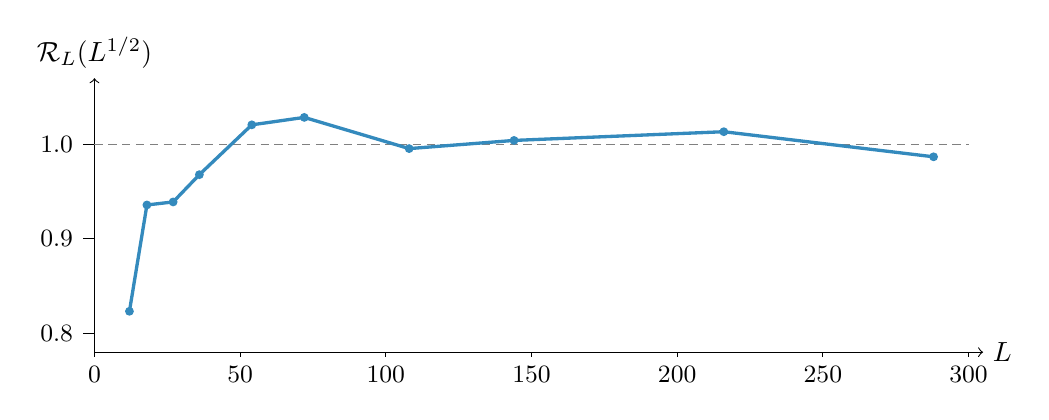
\begin{tikzpicture}[x=0.037cm,y=12cm]
    \draw[->] (0,0.78) -- (305,0.78) node[right] {$L$};
    \draw[->] (0,0.78) -- (0,1.07)
        node[above] {$\calR_L(L^{1/2})$};

    \foreach \x in {0,50,100,150,200,250,300}{
        \draw (\x,0.78) -- (\x,0.775)
            node[below] {\small $\x$};
    }
    \foreach \y in {0.8,0.9,1.0}{
        \draw (0,\y) -- (-4,\y)
            node[left] {\small $\y$};
    }

    \draw[gray,densely dashed] (0,1) -- (300,1);

    \draw[very thick,ct_blue] plot coordinates {
        (12,0.82328)
        (18,0.93581)
        (27,0.93899)
        (36,0.96787)
        (54,1.02060)
        (72,1.02848)
        (108,0.99545)
        (144,1.00411)
        (216,1.01332)
        (288,0.98677)
    };

    \foreach \x/\y in {
        12/0.82328,
        18/0.93581,
        27/0.93899,
        36/0.96787,
        54/1.02060,
        72/1.02848,
        108/0.99545,
        144/1.00411,
        216/1.01332,
        288/0.98677
    }{
        \fill[ct_blue] (\x,\y) circle[radius=1.6pt];
    }
\end{tikzpicture}
\caption{The clean open-chain response evaluated along
$t_L=L^{1/2}$. The dashed line is
$\chi(\Sigma_{E_F})=1$. The residual oscillation reflects finite-time and
finite-volume effects.}
\label{fig:clean thermodynamic sequence}
\end{figure}

\subsection{Boundary conditions}

Open boundary conditions provide the most direct approximation of the
half-line switch. Periodic boundary conditions require additional care.
Consider the ring
\eq{\calH_L^{\mathrm{per}}
:=\ell^2\left(\ZZ/(2L\ZZ)\right)}
and the half-ring projection
\eq{\Lambda_L^{\mathrm{per}}
:=\chi_{\{0,\ldots,L-1\}}(X)\,.}
Unlike the half-line switch, $\Lambda_L^{\mathrm{per}}$ has two interfaces:
one at the bond $(-1,0)$ and another at $(L-1,L)$.

The contributions from the two interfaces add rather than cancel. Indeed,
\eq{\left[
U(1-\Lambda)U^*,1-\Lambda
\right]
=
[U\Lambda U^*,\Lambda]\,.}
Consequently, before the two interfaces communicate,
\eq{\calR_L^{\mathrm{per}}(t)
\simeq 2\calR_L(t)\,.}
The quantity which should be compared with the single-interface open-chain
response is therefore
\eq{\frac{1}{2}\calR_L^{\mathrm{per}}(t)\,.}

\begin{figure}[ht]
\centering
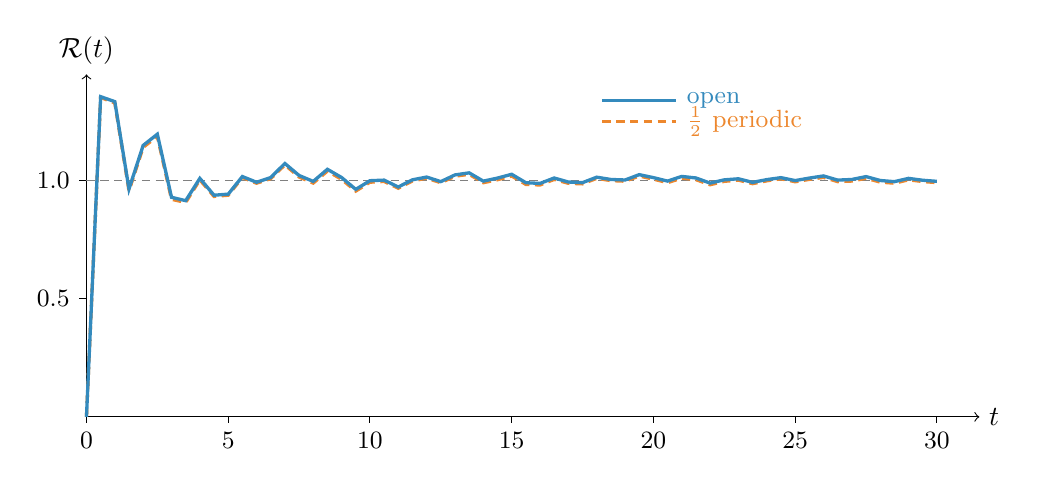
\begin{tikzpicture}[x=0.36cm,y=3cm]
    \draw[->] (0,0) -- (31.5,0) node[right] {$t$};
    \draw[->] (0,0) -- (0,1.45) node[above] {$\calR(t)$};

    \foreach \x in {0,5,10,15,20,25,30}{
        \draw (\x,0) -- (\x,-0.025)
            node[below] {\small $\x$};
    }
    \foreach \y in {0.5,1.0}{
        \draw (0,\y) -- (-0.25,\y)
            node[left] {\small $\y$};
    }

    \draw[gray,densely dashed] (0,1) -- (30,1);

    \draw[very thick,ct_orange,densely dashed] plot coordinates {
      (0.0,0.00000) (0.5,1.35226) (1.0,1.32897)
      (1.5,0.95759) (2.0,1.14100) (2.5,1.18787)
      (3.0,0.92107) (3.5,0.90782) (4.0,1.00352)
      (4.5,0.93320) (5.0,0.93840) (5.5,1.01342)
      (6.0,0.98910) (6.5,1.00858) (7.0,1.06686)
      (7.5,1.01534) (8.0,0.98977) (8.5,1.04055)
      (9.0,1.00569) (9.5,0.95585) (10.0,0.99340)
      (10.5,0.99666) (11.0,0.96810) (11.5,0.99884)
      (12.0,1.01067) (12.5,0.99118) (13.0,1.01888)
      (13.5,1.02690) (14.0,0.99131) (14.5,1.00387)
      (15.0,1.01971) (15.5,0.98416) (16.0,0.98161)
      (16.5,1.00525) (17.0,0.98869) (17.5,0.98646)
      (18.0,1.00980) (18.5,1.00014) (19.0,0.99762)
      (19.5,1.01964) (20.0,1.00640) (20.5,0.99140)
      (21.0,1.01095) (21.5,1.00431) (22.0,0.98270)
      (22.5,0.99712) (23.0,1.00217) (23.5,0.98730)
      (24.0,0.99933) (24.5,1.00775) (25.0,0.99528)
      (25.5,1.00540) (26.0,1.01398) (26.5,0.99587)
      (27.0,0.99823) (27.5,1.01024) (28.0,0.99385)
      (28.5,0.98913) (29.0,1.00353) (29.5,0.99617)
      (30.0,0.99175)
    };

    \draw[very thick,ct_blue] plot coordinates {
      (0.0,0.00000) (0.5,1.35547) (1.0,1.33450)
      (1.5,0.96461) (2.0,1.14911) (2.5,1.19662)
      (3.0,0.92954) (3.5,0.91517) (4.0,1.00957)
      (4.5,0.93829) (5.0,0.94283) (5.5,1.01740)
      (6.0,0.99311) (6.5,1.01328) (7.0,1.07256)
      (7.5,1.02187) (8.0,0.99685) (8.5,1.04802)
      (9.0,1.01327) (9.5,0.96301) (10.0,0.99975)
      (10.5,1.00223) (11.0,0.97315) (11.5,1.00354)
      (12.0,1.01518) (12.5,0.99592) (13.0,1.02426)
      (13.5,1.03302) (14.0,0.99796) (14.5,1.01085)
      (15.0,1.02691) (15.5,0.99128) (16.0,0.98824)
      (16.5,1.01120) (17.0,0.99410) (17.5,0.99153)
      (18.0,1.01464) (18.5,1.00495) (19.0,1.00276)
      (19.5,1.02540) (20.0,1.01272) (20.5,0.99809)
      (21.0,1.01787) (21.5,1.01133) (22.0,0.98952)
      (22.5,1.00342) (23.0,1.00788) (23.5,0.99262)
      (24.0,1.00441) (24.5,1.01269) (25.0,1.00030)
      (25.5,1.01085) (26.0,1.01999) (26.5,1.00232)
      (27.0,1.00493) (27.5,1.01710) (28.0,1.00072)
      (28.5,0.99570) (29.0,1.00956) (29.5,1.00172)
      (30.0,0.99702)
    };

    \fill[white,opacity=0.85] (17.5,1.20)
        rectangle (29.5,1.40);
    \draw[very thick,ct_blue] (18.2,1.34) -- (20.8,1.34)
        node[right] {\small open};
    \draw[very thick,ct_orange,densely dashed]
        (18.2,1.25) -- (20.8,1.25)
        node[right] {\small $\frac12$ periodic};
\end{tikzpicture}
\caption{Comparison at $L=151$. The solid curve is the open-chain
single-interface response. The dashed curve is one half of the periodic
response, which contains two interfaces. The two agree throughout the
pre-recurrence window.}
\label{fig:boundary condition comparison}
\end{figure}

If the exponential cutoff is retained in finite volume, its length scale
must also remain separated from the boundary. A sufficient diagonal
condition is
\eq{\ve_L\downarrow0,\qquad
t_L\to\infty,\qquad
2t_L+\ve_L^{-1}=o(L)\,.}

\subsection{The Anderson model}

We next consider
\eq{H_{\omega,L}
=
H_{0,L}
+
\sum_{n=-L}^{L}\omega_n\ket{n}\bra{n},
\qquad
\omega_n\sim\operatorname{Unif}[-W/2,W/2]}
with $W=3$. For every $W>0$, the one-dimensional Anderson model with a
non-degenerate iid uniform site potential has almost surely pure point
spectrum with exponentially localized eigenfunctions, and its static
conductivity vanishes
\cite{Kunz1980,frohlichConstructiveProofLocalization1985,Anderson_1958_PhysRev.109.1492,MottTwose1961,LeeRamakrishnan1985}.
Thus there is no reason to expect the clean ballistic response to
persist. 

A thermodynamic sequence must nevertheless be constructed before drawing
any conclusion. For every disorder sample, we first generate a potential on
the largest interval and obtain all smaller systems by restriction about the
same origin. Thus the values at different $L$ approximate one fixed infinite
disorder realization rather than unrelated samples.

For $M=200$ disorder realizations, define
\eq{m_L
:=
\frac{1}{M}\sum_{\alpha=1}^{M}
\calR_{\omega_\alpha,L}(L^{1/2})}
and
\eq{s_L
:=
\left(
\frac{1}{M-1}
\sum_{\alpha=1}^{M}
\left|
\calR_{\omega_\alpha,L}(L^{1/2})-m_L
\right|^2
\right)^{1/2}.}
A deterministic samplewise integer would require both
\eq{m_L\longrightarrow m\in\ZZ,
\qquad
s_L\longrightarrow0\,.}

\begin{figure}[ht]
\centering
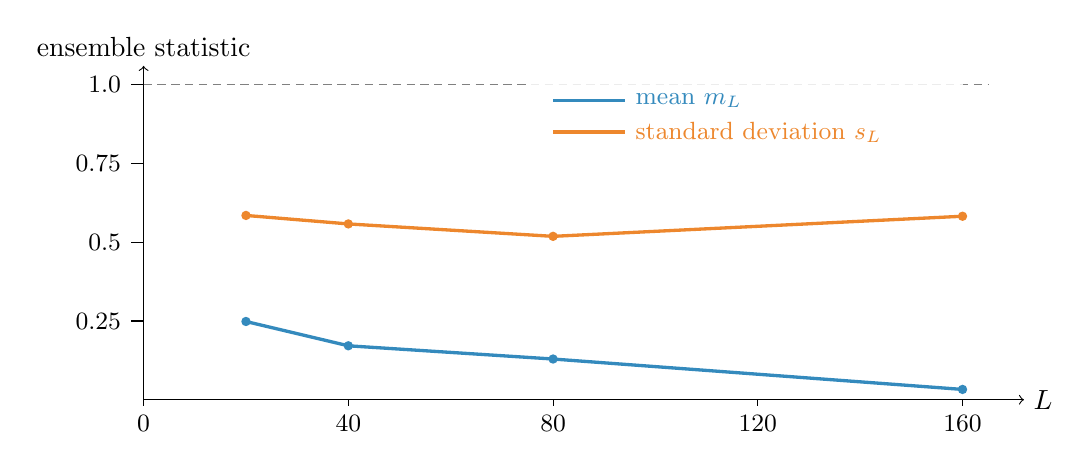
\begin{tikzpicture}[x=0.065cm,y=4cm]
    \draw[->] (0,0) -- (172,0) node[right] {$L$};
    \draw[->] (0,0) -- (0,1.06) node[above] {ensemble statistic};

    \foreach \x in {0,40,80,120,160}{
        \draw (\x,0) -- (\x,-0.02)
            node[below] {\small $\x$};
    }
    \foreach \y in {0.25,0.5,0.75,1.0}{
        \draw (0,\y) -- (-2.5,\y)
            node[left] {\small $\y$};
    }

    \draw[gray,densely dashed] (0,1) -- (165,1);

    \draw[very thick,ct_blue] plot coordinates {
        (20,0.24849)
        (40,0.17132)
        (80,0.12932)
        (160,0.03277)
    };
    \foreach \x/\y in {
        20/0.24849,
        40/0.17132,
        80/0.12932,
        160/0.03277
    }{
        \fill[ct_blue] (\x,\y) circle[radius=1.7pt];
    }

    \draw[very thick,ct_orange] plot coordinates {
        (20,0.58519)
        (40,0.55824)
        (80,0.51882)
        (160,0.58262)
    };
    \foreach \x/\y in {
        20/0.58519,
        40/0.55824,
        80/0.51882,
        160/0.58262
    }{
        \fill[ct_orange] (\x,\y) circle[radius=1.7pt];
    }

    \fill[white,opacity=0.85] (75,0.78)
        rectangle (160,1.02);
    \draw[very thick,ct_blue] (80,0.95) -- (94,0.95)
        node[right] {\small mean $m_L$};
    \draw[very thick,ct_orange] (80,0.85) -- (94,0.85)
        node[right] {\small standard deviation $s_L$};
\end{tikzpicture}
\caption{Anderson scaling at $W=3$, $E_F=1$, and
$t_L=L^{1/2}$, using $M=200$ nested disorder samples. The ensemble mean
moves toward zero, but the sample standard deviation does not decrease.
The data therefore give no evidence for a deterministic samplewise integer.
The dashed line denotes the clean value $1$.}
\label{fig:Anderson scaling}
\end{figure}

The displayed data are compatible with dephasing of the disorder-averaged
response toward zero. They do not establish such a limit. More importantly,
the variance remains of order one over the available sizes. Increasing the
volume removes the artificial boundary but does not spatially average the
disorder near the fixed switch interface. It is therefore possible for the
thermodynamic response to remain sample-dependent and oscillatory even when
its disorder average tends to zero.

%This experiment also explains why a single fixed-volume Anderson curve
%cannot demonstrate a failure of quantization. The relevant questions concern
%the thermodynamic limit of the random response, the behavior of its
%distribution, and only then its long-time asymptotics.

\subsection{Numerical code}

The following code produces all data appearing in
\cref{fig:clean thermodynamic sequence,fig:boundary condition comparison,fig:Anderson scaling}.

\begin{verbatim}
import numpy as np


EF = 1.0


def open_hamiltonian(L, potential=None):
    """Dirichlet Hamiltonian on {-L,...,L}."""
    N = 2 * L + 1
    H = (
        2 * np.eye(N)
        - np.eye(N, k=1)
        - np.eye(N, k=-1)
    )
    if potential is not None:
        H = H + np.diag(potential)
    return H


def periodic_hamiltonian(L):
    """Clean Hamiltonian on Z/(2L Z)."""
    N = 2 * L
    H = (
        2 * np.eye(N)
        - np.eye(N, k=1)
        - np.eye(N, k=-1)
    )
    H[0, -1] = -1
    H[-1, 0] = -1
    return H


def open_switch(L):
    """Indicator of {0,...,L} in {-L,...,L}."""
    return (
        np.arange(2 * L + 1) >= L
    ).astype(float)


def periodic_switch(L):
    """Indicator of one half of the ring."""
    switch = np.zeros(2 * L)
    switch[:L] = 1.0
    return switch


def response(H, switch, times):
    """
    Return the finite-volume response at every time.

    The complete eigensystem is required.
    """
    times = np.atleast_1d(times)

    energies, vectors = np.linalg.eigh(H)
    occupied = energies < EF

    switch_eigenbasis = (
        vectors.conj().T
        @ (switch[:, None] * vectors)
    )

    gaps = (
        energies[~occupied][None, :]
        - energies[occupied][:, None]
    )
    weights = (
        4 * np.pi
        * np.abs(
            switch_eigenbasis[
                np.ix_(occupied, ~occupied)
            ]
        )**2
    )

    phases = np.sin(
        times[:, None, None] * gaps[None, :, :]
    )
    return np.einsum(
        "tab,ab->t", phases, weights
    )


# --------------------------------------------------
# 1. Clean thermodynamic sequence
# --------------------------------------------------

clean_sizes = np.array([
    12, 18, 27, 36, 54,
    72, 108, 144, 216, 288
])

clean_diagonal = np.empty(len(clean_sizes))

for j, L in enumerate(clean_sizes):
    time = np.sqrt(L)
    clean_diagonal[j] = response(
        open_hamiltonian(L),
        open_switch(L),
        np.array([time]),
    )[0]

print("clean diagonal sequence")
print(np.column_stack((
    clean_sizes,
    np.sqrt(clean_sizes),
    clean_diagonal,
)))


# --------------------------------------------------
# 2. Open versus periodic boundary conditions
# --------------------------------------------------

boundary_L = 151
boundary_times = np.arange(0.0, 30.1, 0.5)

open_curve = response(
    open_hamiltonian(boundary_L),
    open_switch(boundary_L),
    boundary_times,
)

periodic_curve = response(
    periodic_hamiltonian(boundary_L),
    periodic_switch(boundary_L),
    boundary_times,
)

# The periodic switch has two interfaces.
periodic_per_interface = periodic_curve / 2

print("boundary-condition comparison")
print(np.column_stack((
    boundary_times,
    open_curve,
    periodic_per_interface,
)))


# --------------------------------------------------
# 3. Anderson thermodynamic sequence
# --------------------------------------------------

disorder_strength = 3.0
anderson_sizes = np.array([20, 40, 80, 160])
number_of_samples = 200
largest_L = int(anderson_sizes[-1])

anderson_values = np.empty((
    number_of_samples,
    len(anderson_sizes),
))

for sample in range(number_of_samples):
    rng = np.random.default_rng(1000 + sample)

    # One realization on the largest interval.
    full_potential = rng.uniform(
        -disorder_strength / 2,
        disorder_strength / 2,
        2 * largest_L + 1,
    )

    for j, L_value in enumerate(anderson_sizes):
        L = int(L_value)

        # Restrict the same realization about the origin.
        potential = full_potential[
            largest_L - L:
            largest_L + L + 1
        ]

        anderson_values[sample, j] = response(
            open_hamiltonian(L, potential),
            open_switch(L),
            np.array([np.sqrt(L)]),
        )[0]

anderson_mean = anderson_values.mean(axis=0)
anderson_std = anderson_values.std(
    axis=0, ddof=1
)
anderson_standard_error = (
    anderson_std / np.sqrt(number_of_samples)
)

print("Anderson ensemble statistics")
print(np.column_stack((
    anderson_sizes,
    anderson_mean,
    anderson_std,
    anderson_standard_error,
)))
\end{verbatim}

For reference, the last block gives
\eq{
\begin{array}{c|cccc}
L & 20 & 40 & 80 & 160\\ \hline
m_L
&0.24849&0.17132&0.12932&0.03277\\
s_L
&0.58519&0.55824&0.51882&0.58262
\end{array}}
The standard errors of the four displayed means are, respectively,
$0.04138$, $0.03947$, $0.03669$, and $0.04120$.
  
  \begingroup
		\let\itshape\upshape
		\printbibliography
		\endgroup
	
    
    
    \end{document}
